\section{Homework 1}

\subsection{Il gioco}
Nel primo homework andremo ad analizzare il gioco del \textbf{Sasso, carta, forbici, spok e lizard}. Il gioco è molto semplice ed è implementato nel file \code{spok.m} nella cartella \code{homeworks/1 spok}: l'agente chiama la funzione \code{spok} con la sua mossa e la funzione ritorna il reward ottenuto, secondo lo schema seguente.

\begin{center}
\begin{tabular}{cl}
\toprule
\textbf{Reward} & \textbf{Esito} \\
\midrule
$+1$ & vincita \\
$-1$ & sconfitta \\
\bottomrule
\end{tabular}
\end{center}

Le mosse possibili sono 5 e sono mappate come segue:

\begin{center}
\begin{tabular}{ccccc}
\toprule
1 & 2 & 3 & 4 & 5 \\
\midrule
sasso & carta & forbice & lizard & spok \\
\bottomrule
\end{tabular}
\end{center}


Il gioco è implementato in modo da essere \textbf{equo}: ogni mossa ha la stessa probabilità di vincere o perdere contro le altre. È tuttavia possibile renderlo \textbf{non equo} passando alla funzione \code{spok} un parametro booleano: in tal caso l'avversario gioca \emph{spok} con probabilità $60\%$, distribuendo equamente la probabilità restante tra le altre mosse.


Gli algoritmi di reinforcement learning utilizzati dall'agente sono tutti relativi al \emph{bandit problem}.

\subsection{Algoritmi}

\subsubsection{Sample average}
I primi due algoritmi si basano sul concetto di \emph{sample average} della reward ottenuta:
\[
Q_{t+1}(a) = Q_t(a) + \alpha\big(R_t - Q_t(a)\big)
\]

\paragraph{$\epsilon$-greedy.} Con probabilità $\epsilon$ l'agente sceglie una mossa a caso, mentre con probabilità $1-\epsilon$ sceglie la mossa con il valore di $Q$ più alto.
\begin{infobox}[Parametri]
\begin{itemize}[nosep]
    \item $\epsilon = 0.1$
    \item $\alpha = 1/n(s,a)$, cioè l'inverso del numero di volte che quella mossa è stata scelta
\end{itemize}
\end{infobox}

\paragraph{UCB (Upper Confidence Bound).} L'agente sceglie la mossa con il valore di $Q$ più alto, sommato a un termine di esplorazione che dipende dal numero di volte che quella mossa è stata scelta in passato:
\[
Q_t(a) + c\sqrt{\frac{\ln(t)}{n(s,a)}}
\]
\begin{infobox}[Parametri]
\begin{itemize}[nosep]
    \item $c = 10$
    \item $\alpha = 0.0001$ (costante)
\end{itemize}
\end{infobox}

\subsubsection{Preference update}
L'ultimo algoritmo si basa sul concetto di \emph{preferenze}: l'agente mantiene un vettore di preferenze $H(a)$ per ogni mossa e adotta una politica \emph{softmax}, scegliendo ciascuna mossa con probabilità proporzionale alla sua preferenza:
\[
P(a) = \frac{e^{H(a)}}{\sum_{b} e^{H(b)}}
\]
Ad ogni passo tutte le preferenze vengono aggiornate in base alla reward ottenuta: la preferenza della mossa scelta viene aumentata proporzionalmente alla reward, mentre le altre vengono diminuite proporzionalmente alla stessa:
\begin{align}
    &H_{t+1}(a)=H_t(a) + \alpha (R_t - \overline{R_t})(1-P_t(a)) \\
    &H_{t+1}(b)=H_t(b) - \alpha (R_t - \overline{R_t})P_t(b) \quad \forall b\neq a
\end{align}

Dove $\overline{R_t}$ è la media delle reward ottenute fino a quel momento.
\begin{infobox}[Parametri]
\begin{itemize}[nosep]
    \item $\alpha = 0.0001$
\end{itemize}
\end{infobox}

\subsection{Risultati}
I risultati riportati di seguito sono stati calcolati su $10^6$ partite simulate.

\subsubsection*{Gioco equo}
\begin{infobox}[Aspettative]
Con mosse dell'avversario equiprobabili, nessun algoritmo dovrebbe riuscire a individuare una mossa migliore delle altre: per i due algoritmi a \emph{sample average} la distribuzione delle reward per mossa dovrebbe restare uniforme e centrata attorno allo zero; per l'algoritmo a preferenze, tutte le preferenze dovrebbero stabilizzarsi attorno allo stesso valore.
\end{infobox}

Nell'immagine \ref{fig:fair_game_h1} sono riportati i risultati ottenuti per i tre algoritmi: sull'asse delle ascisse è riportato l'avanzare del tempo (numero di partite giocate), su quello delle ordinate il valore della funzione utilizzata dall'agente ($Q$ o $H$). I risultati sono coerenti con le aspettative: le funzioni $Q$ e $H$ si stabilizzano tutte attorno allo stesso valore, senza che una mossa prevalga sulle altre. Per il secondo e il terzo algoritmo si nota come un $\alpha$ costante, per quanto piccolo, porti a una maggiore variabilità dei valori di $Q$ e $H$ rispetto al primo algoritmo, dove $\alpha$ è decrescente e proporzionale al numero di volte che una mossa è stata scelta. Questa variabilità è ancora più evidente nel terzo grafico, poiché le preferenze partono da $0$, mentre la funzione $Q$ per UCB parte da un valore grande per eliminare il bias iniziale; nel caso $\epsilon$-greedy parte invece da $0$, ma viene aggiornata con un $\alpha$ decrescente che porta a una stabilizzazione più rapida.

\begin{figure}[htbp]
    \centering
    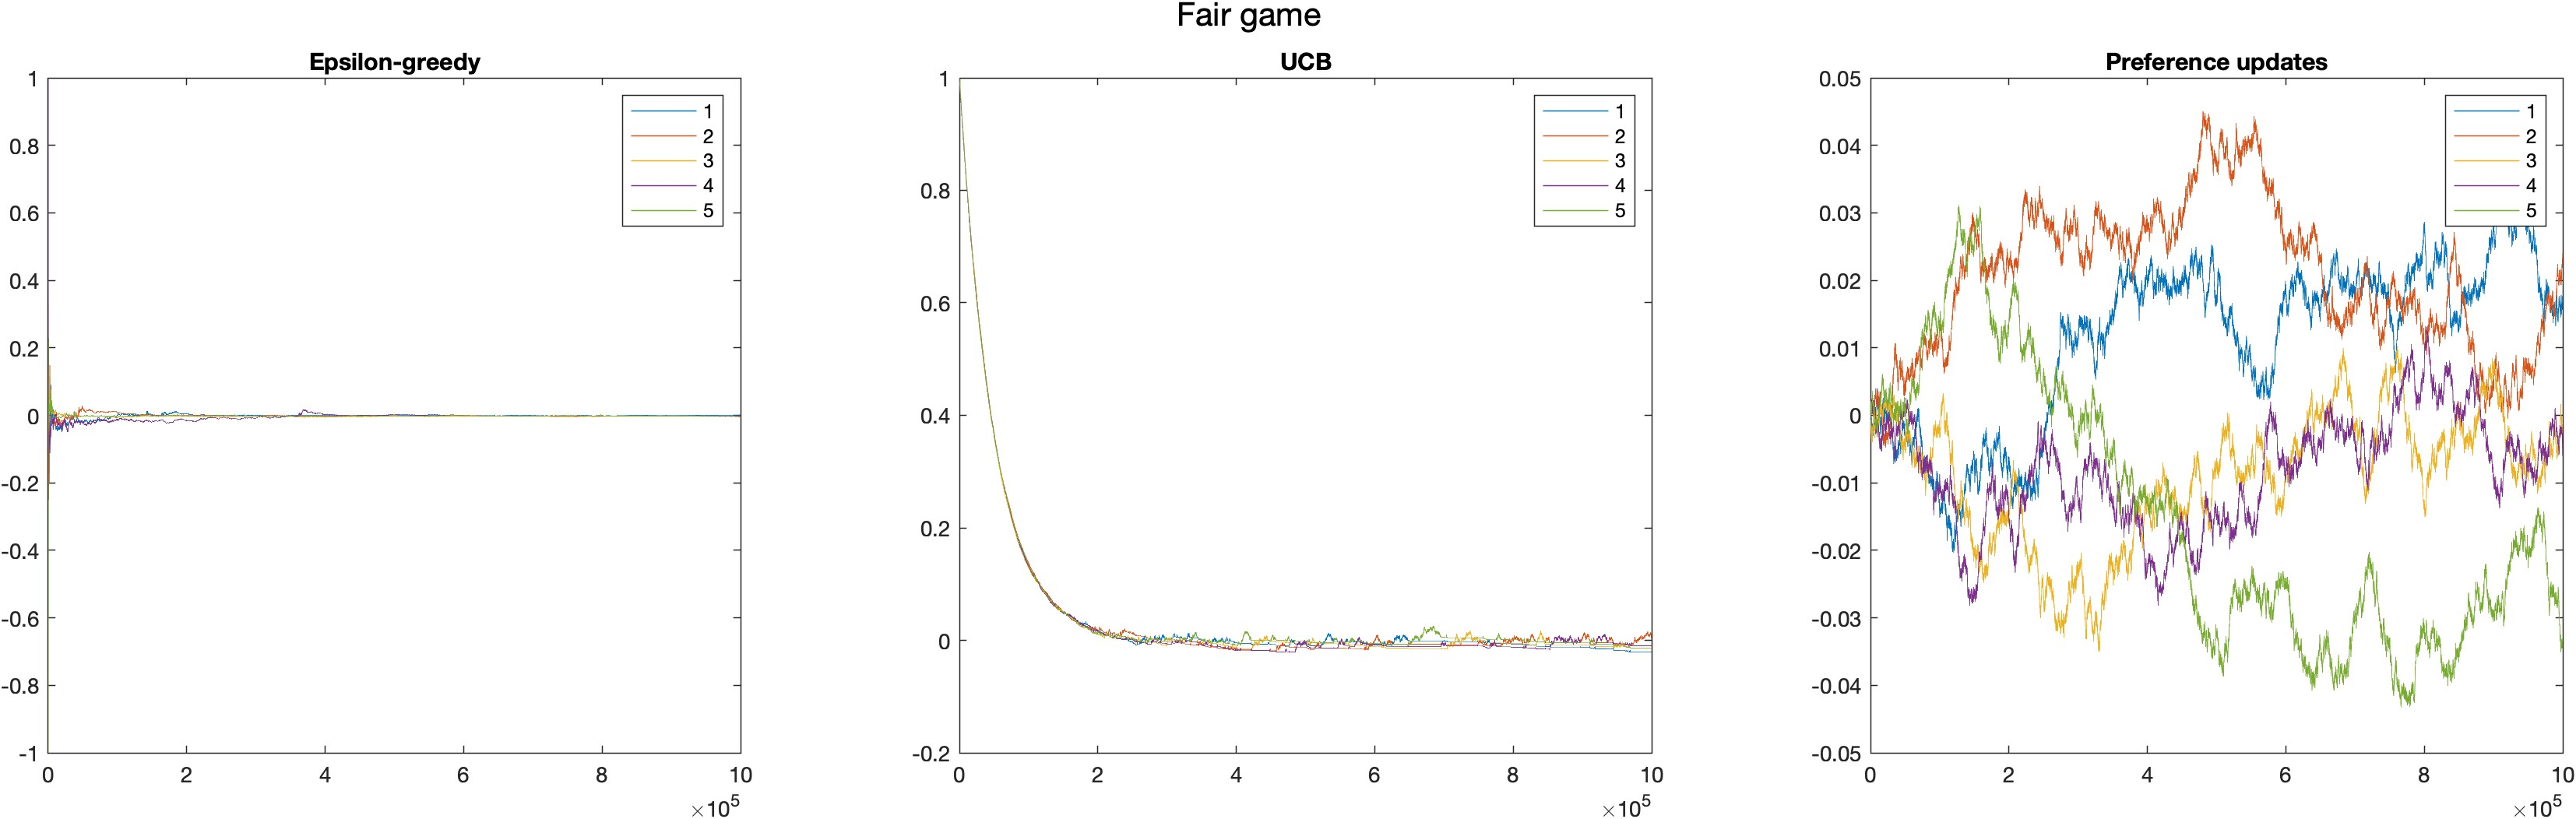
\includegraphics[width=1\textwidth]{homeworks/1/img/fair_game.jpg}
    \caption{Fair game}\label{fig:fair_game_h1}
\end{figure}

\subsubsection*{Gioco non equo}
\begin{infobox}[Aspettative]
Favorendo la mossa $5$ (spok), l'agente deve imparare che esistono ora mosse favorevoli ($2$ e $4$) e mosse sfavorevoli ($1$ e $3$). Per i due algoritmi a \emph{sample average} ci si aspetta che imparino a preferire le mosse favorevoli in base alla reward attesa; per l'algoritmo a preferenze, che le preferenze delle mosse favorevoli aumentino e quelle delle mosse sfavorevoli diminuiscano.
\end{infobox}

I risultati, riportati in figura \ref{fig:unfair_game_h1}, confermano le aspettative: le mosse favorevoli assumono un valore di $Q$ tra $0.5$ e $0.6$, quelle sfavorevoli tra $-0.5$ e $-0.6$; nell'algoritmo a preferenze, le preferenze delle mosse favorevoli aumentano e quelle delle mosse sfavorevoli diminuiscono, come atteso.

\begin{figure}[htbp]
    \centering
    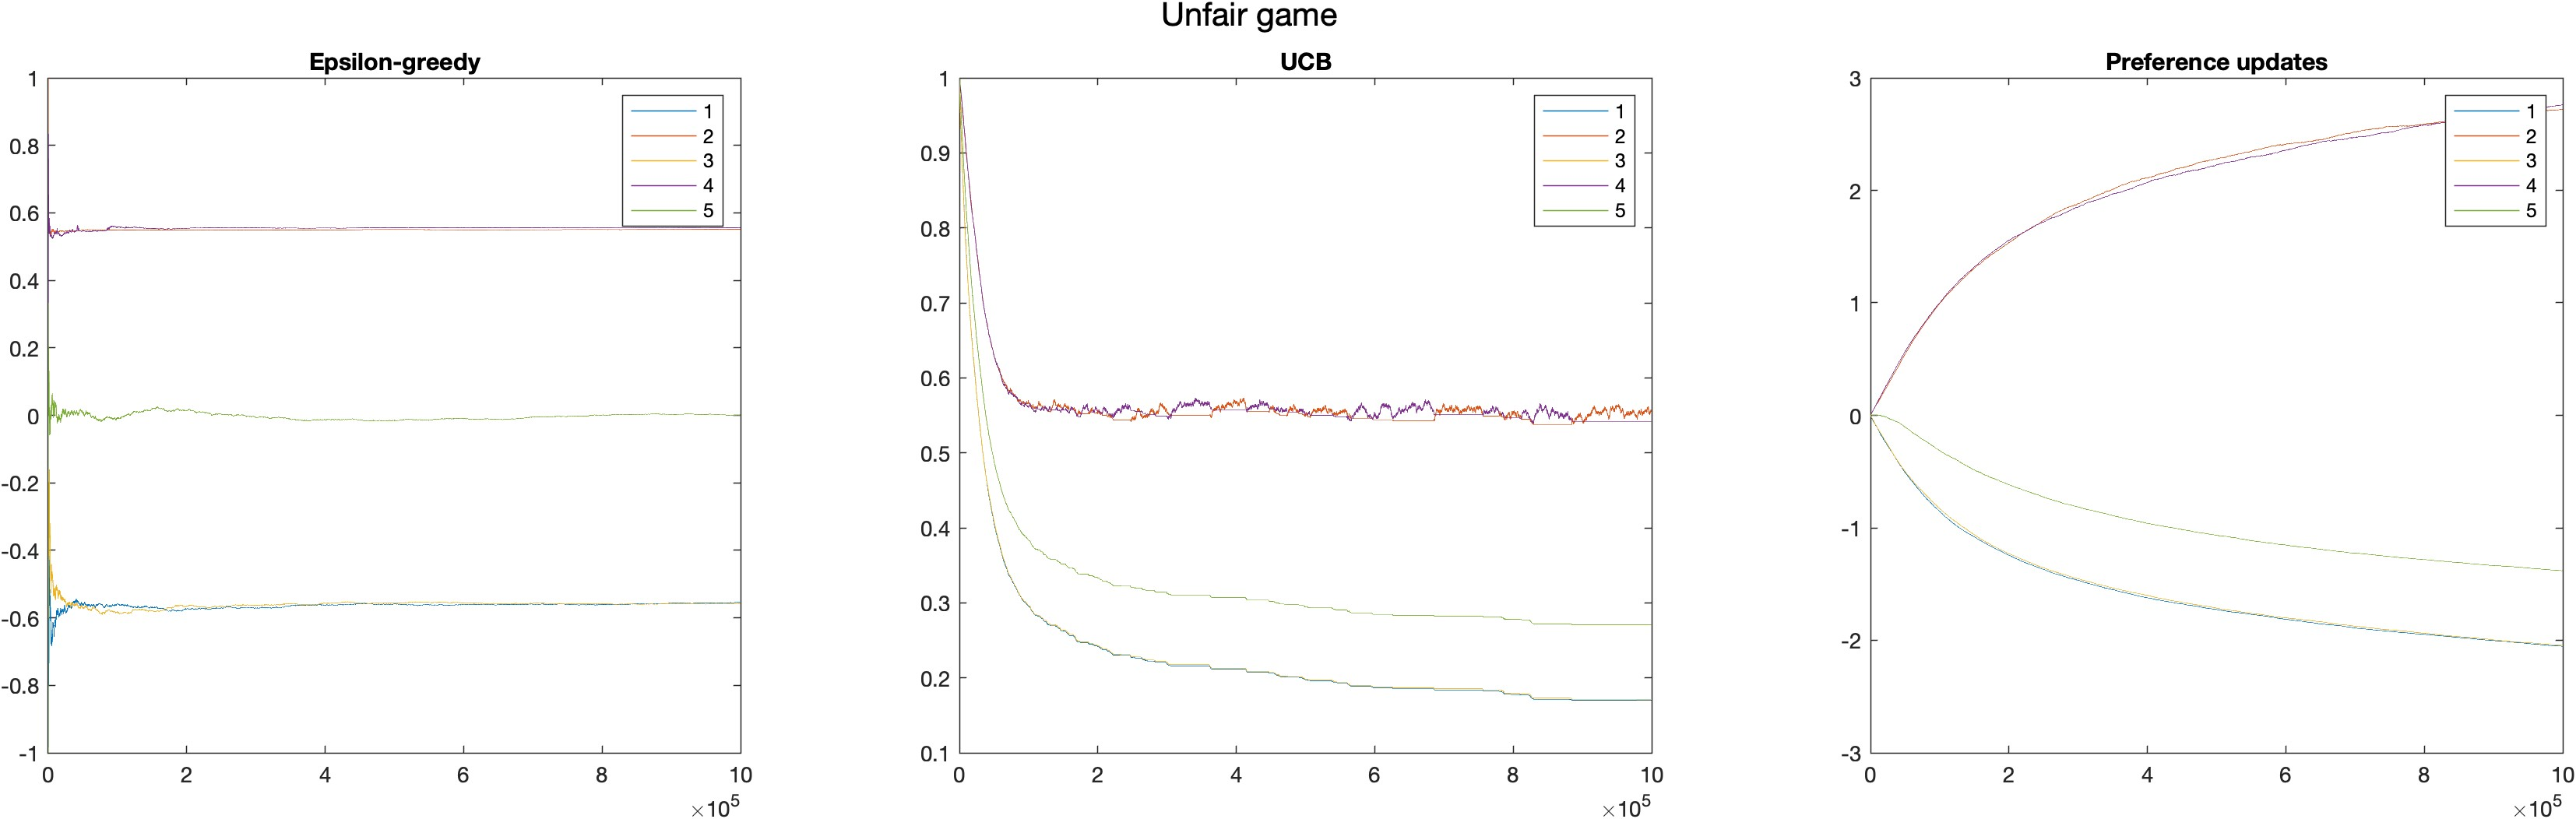
\includegraphics[width=1\textwidth]{homeworks/1/img/unfair_game.jpg}
    \caption{Unfair game}\label{fig:unfair_game_h1}
\end{figure}

Il grafico della UCB, pur mostrando un andamento simile a quello di $\epsilon$-greedy per le mosse favorevoli, si comporta diversamente per le mosse $5$, $1$ e $3$: poiché $Q$ rappresenta un valore atteso di reward, un valore positivo per queste mosse sarebbe matematicamente impossibile. Questa rappresentazione distorta è dovuta al fatto che nell'algoritmo UCB $\alpha$ è costante e molto basso, il che rende la convergenza molto lenta; alzarlo avrebbe reso il grafico molto più instabile, per cui si è preferito mantenere un $\alpha$ basso a costo di una convergenza lenta. Per verificare che il comportamento finale sarebbe stato comunque coerente con il caso $\epsilon$-greedy, è stato eseguito un test con $\alpha$ decrescente: il risultato, mostrato in figura \ref{fig:late_ucb}, conferma le aspettative.

\begin{figure}[htbp]
    \centering
    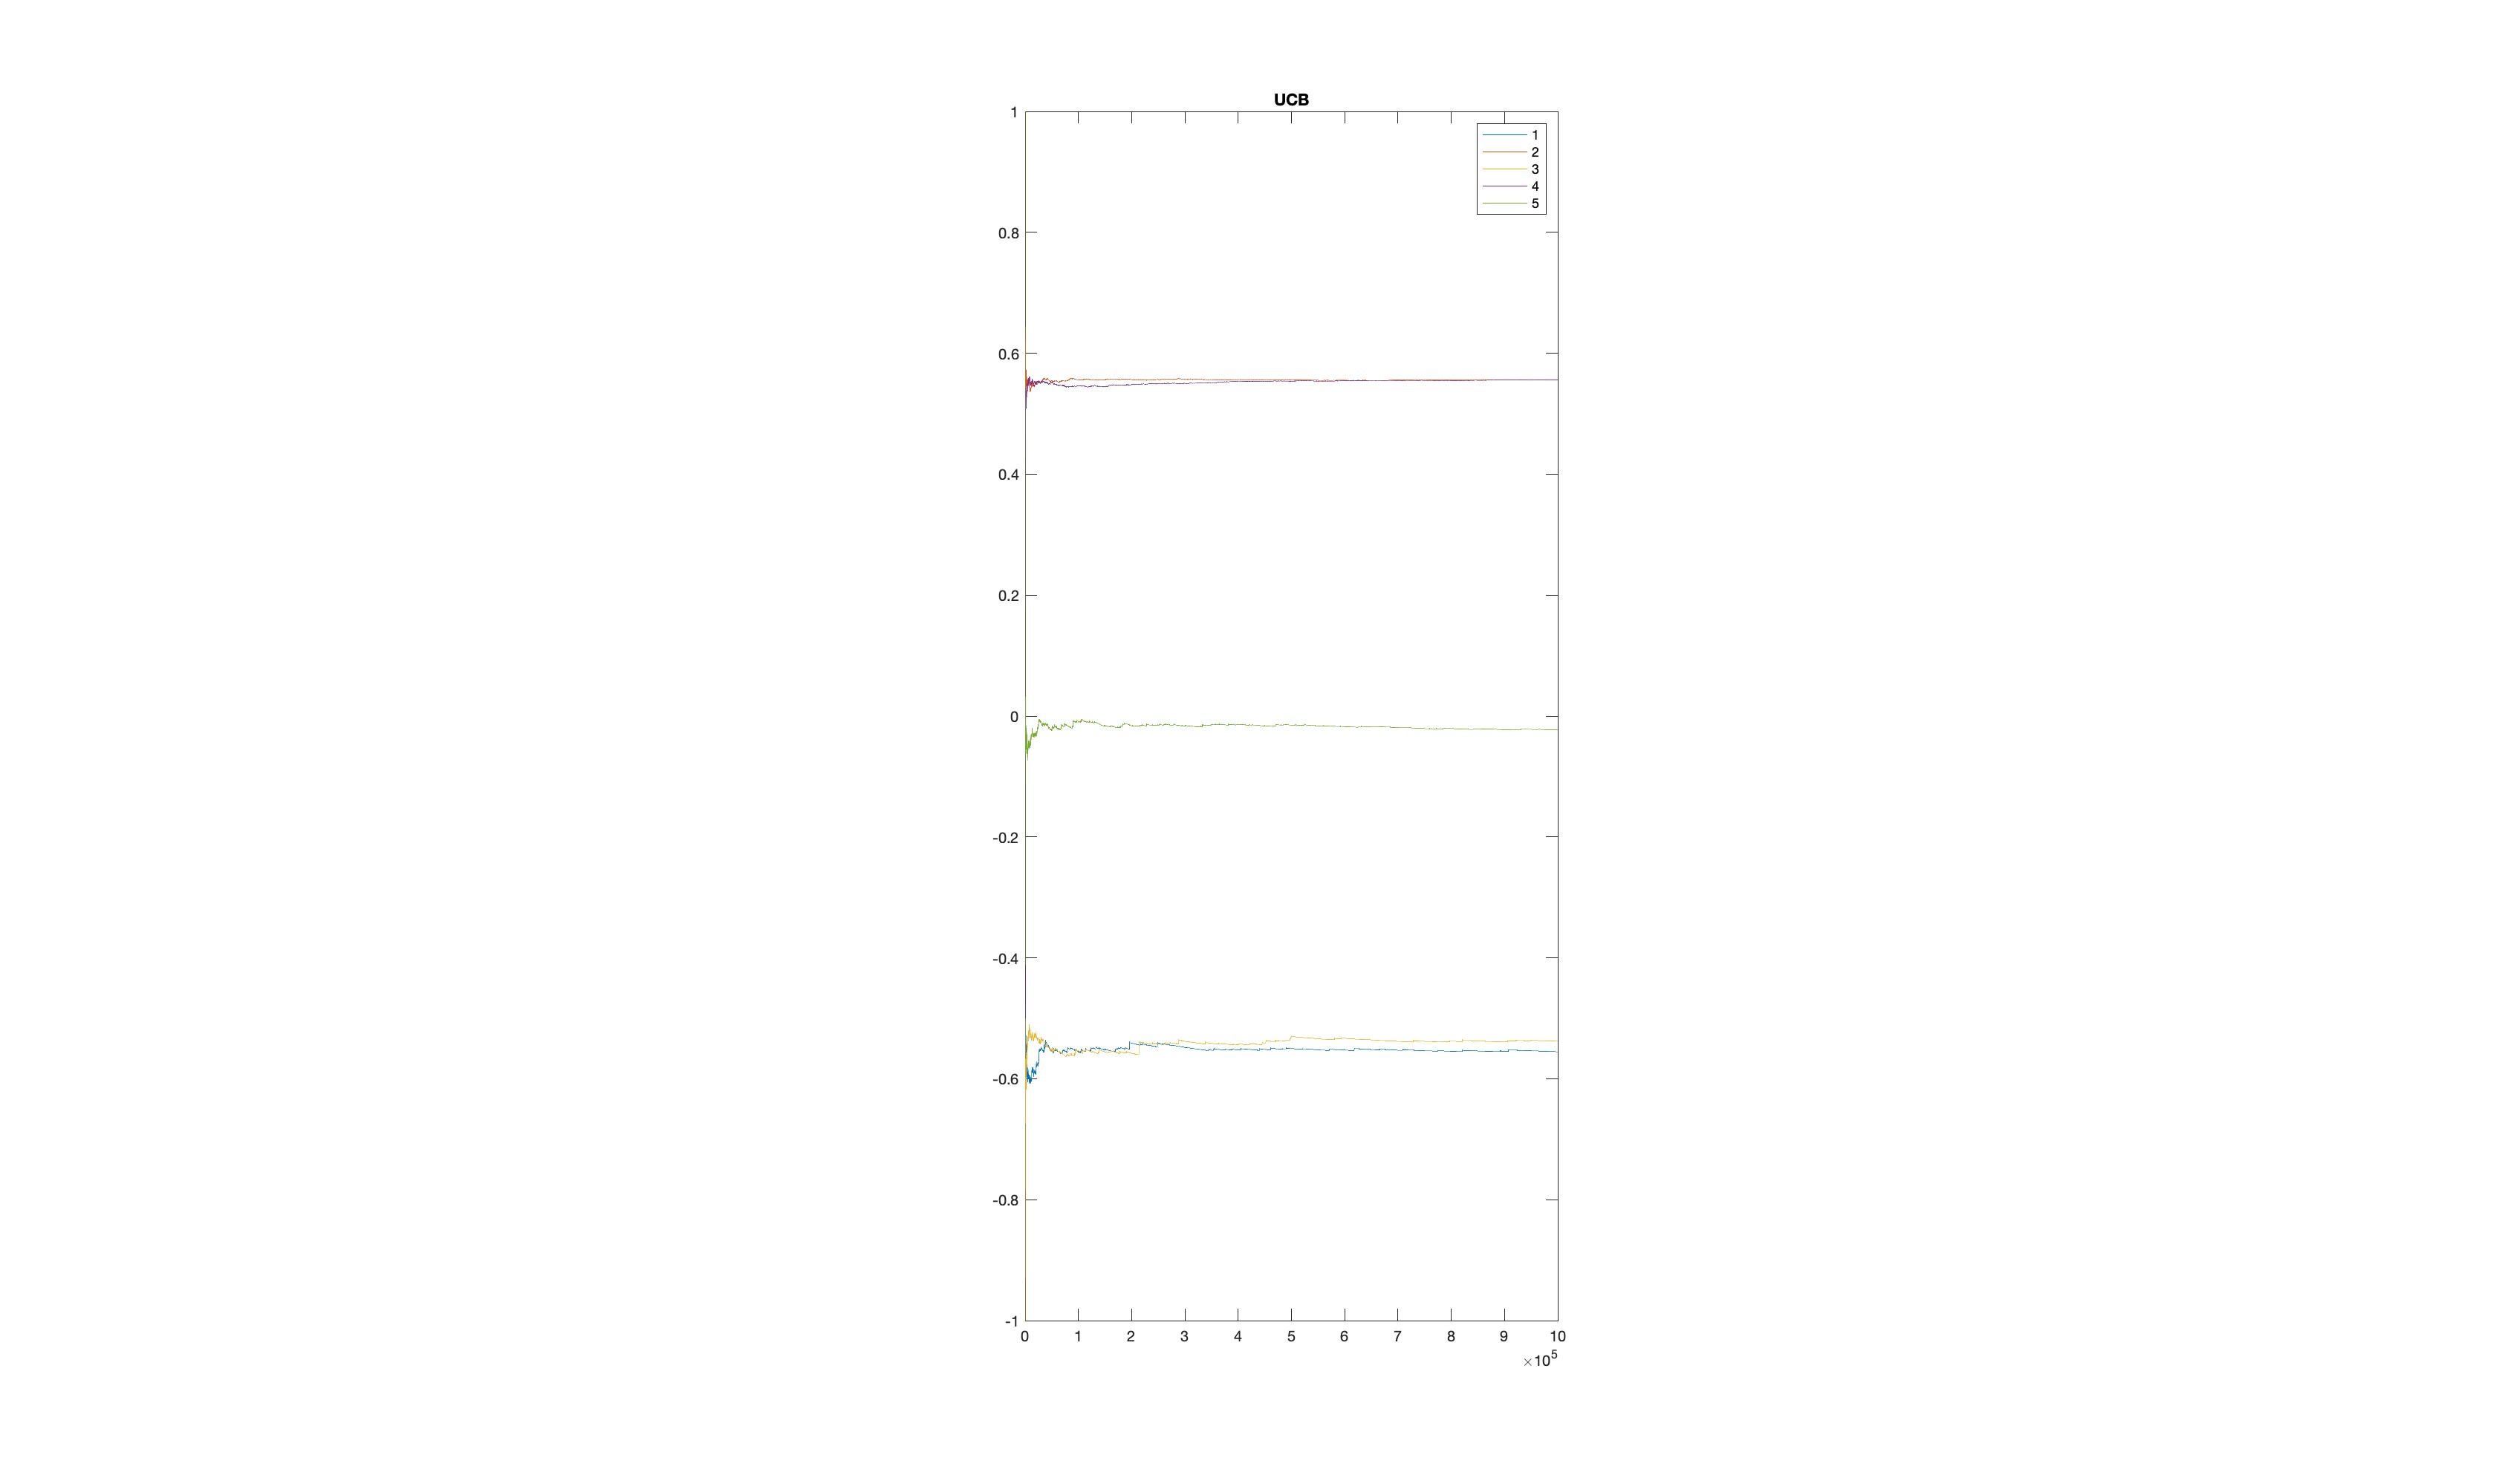
\includegraphics[width=1\textwidth]{homeworks/1/img/ucb_n.jpg}
    \caption{UCB con $\alpha$ decrescente}\label{fig:late_ucb}
\end{figure}

\subsubsection*{Gioco non equo con ritardo}
\begin{infobox}[Aspettative]
In questo scenario la componente \emph{unfair} del gioco viene introdotta a metà simulazione: l'obiettivo è verificare se i vari algoritmi siano in grado di adattare la propria strategia una volta che le probabilità cambiano.
\end{infobox}

Come mostrato in figura \ref{fig:late_unfair_game_h1}, tutti e tre gli algoritmi riescono a modificare la propria strategia, ma solo l'algoritmo a preferenze individua entrambe le mosse migliori; gli altri due si fermano a una sola. Per $\epsilon$-greedy ciò è dovuto al fatto che $\alpha$ è decrescente: una volta individuata una mossa migliore, l'esplorazione necessaria per trovarne una seconda richiederebbe un numero di partite molto elevato. Per UCB la causa è duplice: il termine di esplorazione diminuisce con il tempo, e $\alpha$ è costante e molto basso, per cui la funzione $Q$ non riesce a variare rapidamente. L'algoritmo a preferenze, invece, è più sensibile ai cambiamenti della reward e riesce quindi ad aggiornare le proprie preferenze più velocemente, trovando entrambe le mosse migliori. Modificando opportunamente i parametri sarebbe possibile far individuare entrambe le mosse migliori anche agli altri due algoritmi; si è tuttavia scelto di mantenere i parametri usati in precedenza, per osservare il comportamento degli algoritmi in un caso più realistico.

\begin{figure}[htbp]
    \centering
    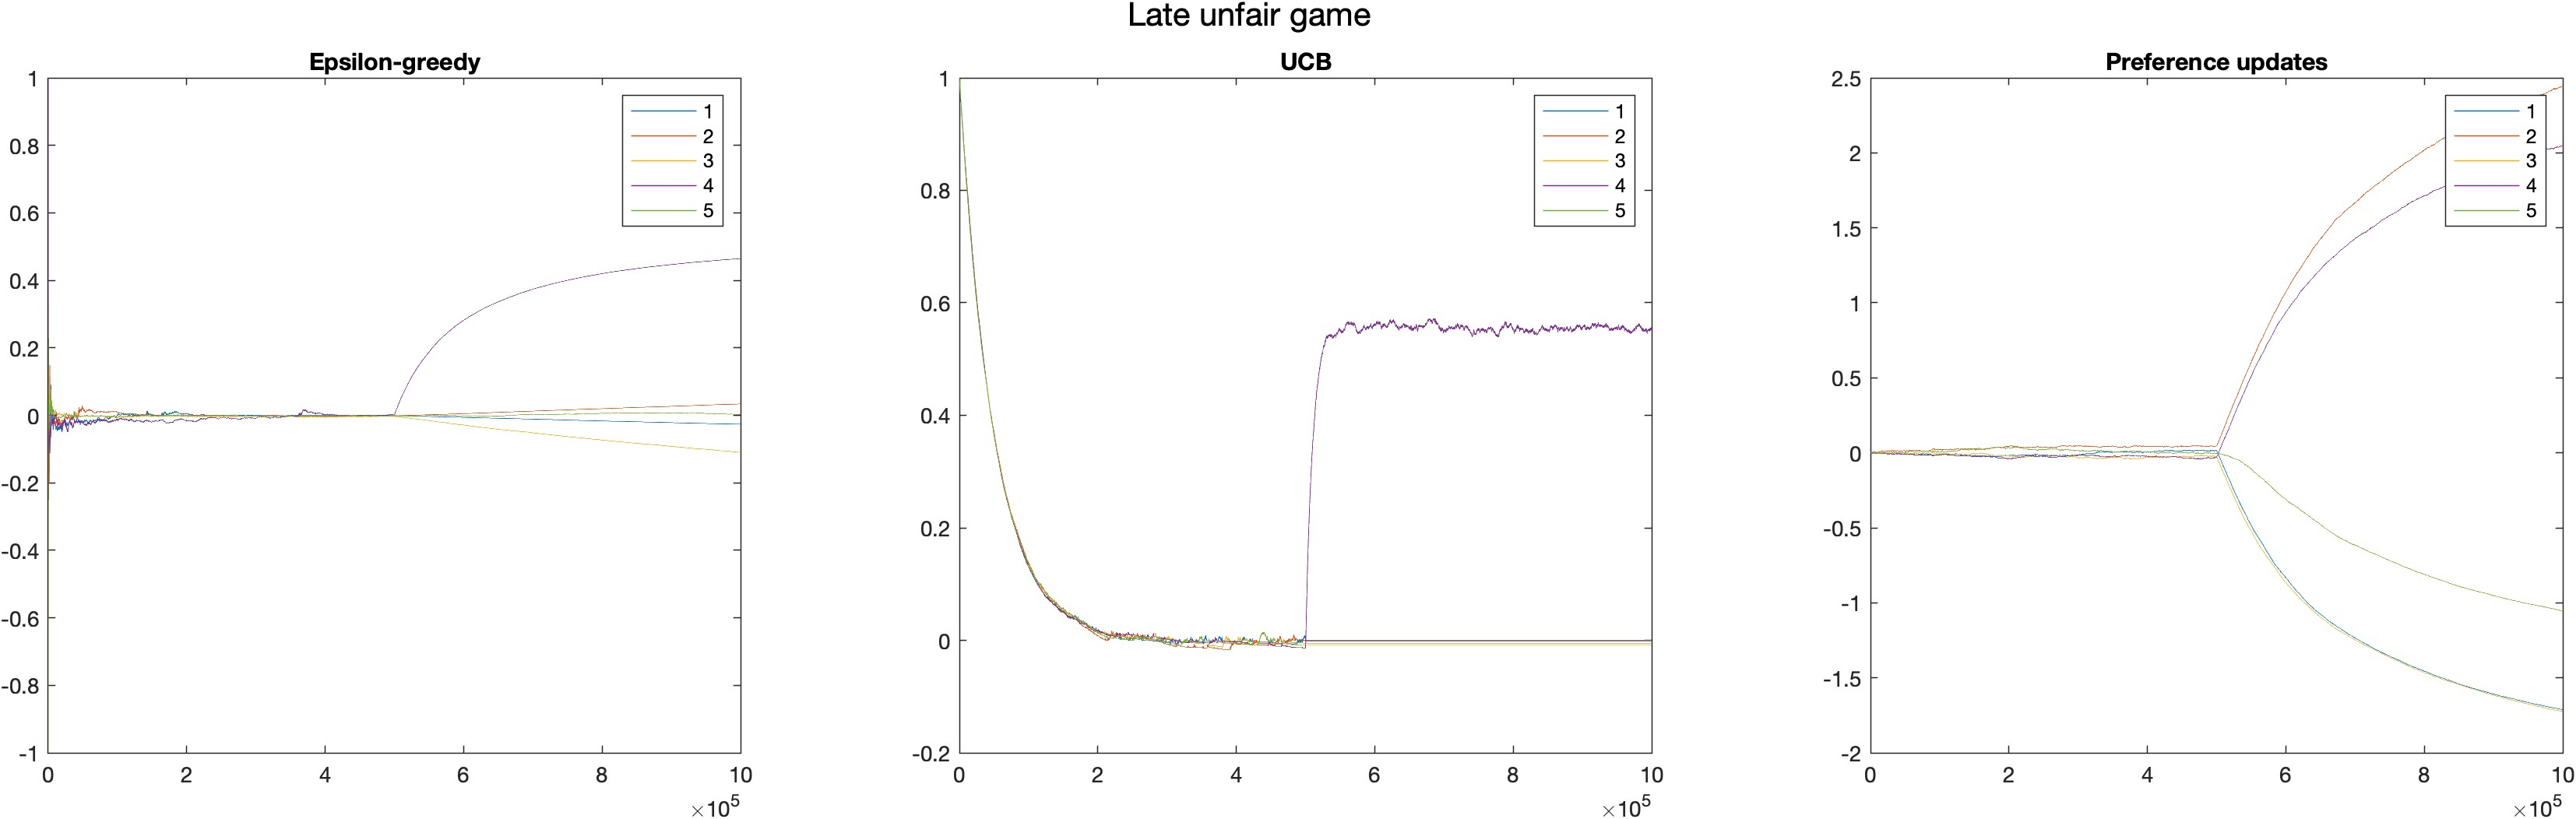
\includegraphics[width=1\textwidth]{homeworks/1/img/late_unfair_game.jpg}
    \caption{Late unfair game}\label{fig:late_unfair_game_h1}
\end{figure}